\documentclass{standalone}
\usepackage[T1]{fontenc}
\usepackage[utf8]{inputenc}
\usepackage[auto]{microtype}
%\usepackage{cmbright}
\usepackage{arev}
\usepackage{amsmath, amssymb, amsfonts, icomma}
\usepackage[version=4]{mhchem}
\usepackage{tikz}
\usepackage{chemplants-tub}
\usepackage{xcolor}
%define stream tip, default is stealth
\setchpstreamtip{latex}
\setchpmainstreamthickness{thick}
%\setchpunitthickness{very thick}

\pgfdeclarelayer{bg}    % declare background layer
\pgfsetlayers{bg,main}  % set the order of the layers (main is the standard layer)

% TABLEAU-10
\definecolor{Tab10-A}{RGB}{78, 121, 167}
\definecolor{Tab10-B}{RGB}{242, 142, 43}
\definecolor{Tab10-C}{RGB}{225, 87, 89}
\definecolor{Tab10-D}{RGB}{118, 183, 178}
\definecolor{Tab10-E}{RGB}{89, 161, 79}
\definecolor{Tab10-F}{RGB}{237, 201, 72}
\definecolor{Tab10-G}{RGB}{176, 122, 161}
\definecolor{Tab10-H}{RGB}{255, 157, 167}
\definecolor{Tab10-I}{RGB}{156, 117, 95}
\definecolor{Tab10-J}{RGB}{186, 176, 172}

\definecolor{AC}{RGB}{74, 84, 106}

\begin{document}
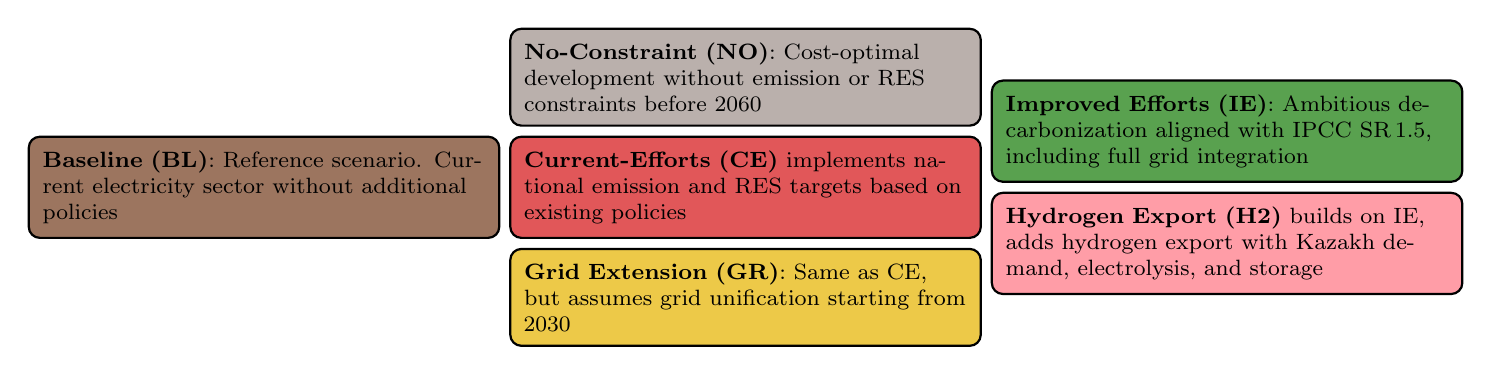
\begin{tikzpicture}[font=\footnotesize]

\node [rectangle, rounded corners, draw=black, fill=Tab10-I, minimum width=140pt, text width= 160pt, thick, inner sep=5pt, outer sep=2pt, align=left] (bl) at (1,1) {\textbf{Baseline (BL)}: Reference scenario. Current electricity sector without additional policies};

\node [rectangle, rounded corners, draw=black, fill=Tab10-J, minimum width=140pt, text width= 160pt, thick, inner sep=5pt, outer sep=2pt, align=left, anchor=south west] (no) at (bl.north east) {
\textbf{No-Constraint (NO)}: Cost-optimal development without emission or RES constraints before 2060};

\node [rectangle, rounded corners, draw=black, fill=Tab10-C, minimum width=140pt, text width= 160pt, thick, inner sep=5pt, outer sep=2pt, align=left, anchor=west, right] (ce) at (bl.east) {
\textbf{Current-Efforts (CE)} implements national emission and RES targets based on existing policies};

\node [rectangle, rounded corners, draw=black, fill=Tab10-F, minimum width=140pt, text width= 160pt, thick, inner sep=5pt, outer sep=2pt, align=left, anchor=north, below] (gr) at (ce.south) {
\textbf{Grid Extension (GR)}: Same as CE, but assumes grid unification starting from 2030};

\node [rectangle, rounded corners, draw=black, fill=Tab10-E, minimum width=140pt, text width= 160pt, thick, inner sep=5pt, outer sep=2pt, align=left, anchor=west, right] (ie) at (ce.north east) {
\textbf{Improved Efforts (IE)}: Ambitious decarbonization aligned with IPCC SR\,1.5, including full grid integration};

\node [rectangle, rounded corners, draw=black, fill=Tab10-H, minimum width=140pt, text width= 160pt, thick, inner sep=5pt, outer sep=2pt, align=left, anchor=north, below] (h2) at (ie.south) {
\textbf{Hydrogen Export (H2)}  
    builds on IE, adds hydrogen export with Kazakh demand, electrolysis, and storage};

\end{tikzpicture}

\end{document}